\documentclass[tikz,border=10pt]{standalone}
\usetikzlibrary{calc}
\begin{document}
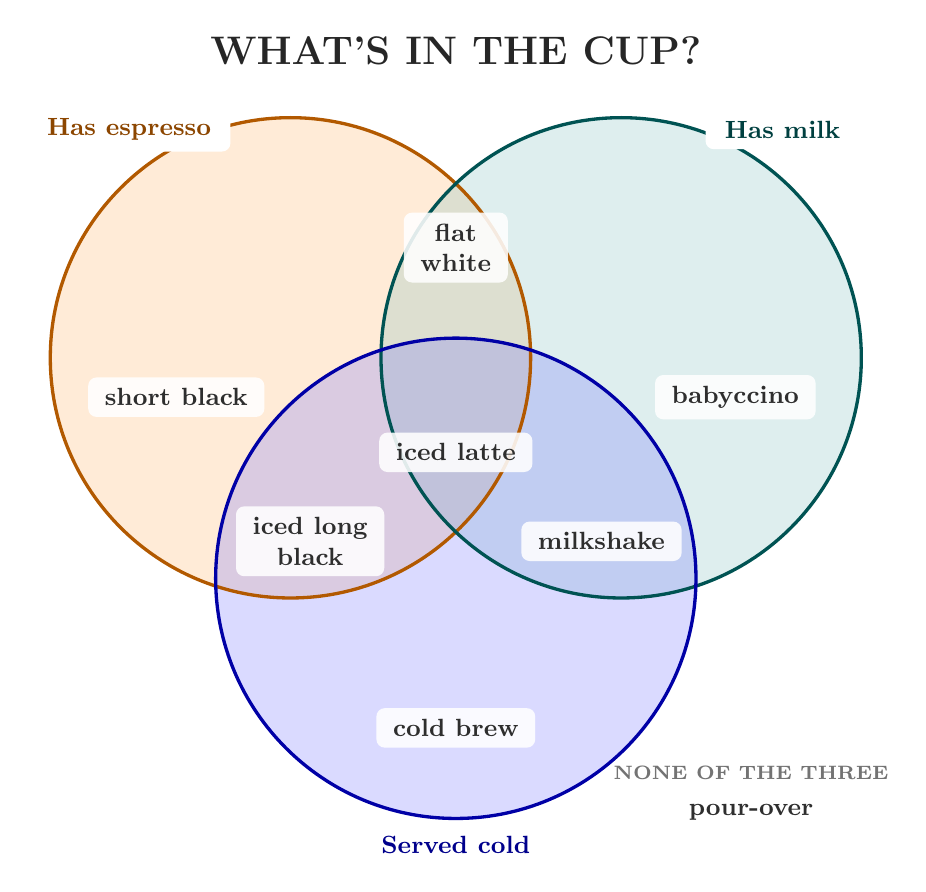
\begin{tikzpicture}[font=, every node/.style={text=black!82}]
  % A soft, overlapping palette keeps all seven interior regions legible.
  \fill[orange!65, fill opacity=.24] (-2.1,1.15) circle (3.05);
  \fill[teal!55, fill opacity=.24] (2.1,1.15) circle (3.05);
  \fill[blue!60, fill opacity=.24] (0,-1.65) circle (3.05);
  \draw[orange!70!black, line width=1.2pt] (-2.1,1.15) circle (3.05);
  \draw[teal!65!black, line width=1.2pt] (2.1,1.15) circle (3.05);
  \draw[blue!65!black, line width=1.2pt] (0,-1.65) circle (3.05);

  \node[font=\bfseries\Large, text=black!85] at (0,5.05) {WHAT'S IN THE CUP?};
  \node[font=\bfseries\small, fill=white, rounded corners=3pt,
        inner xsep=7pt, inner ysep=4pt, text=orange!55!black] at (-4.15,4.05) {Has espresso};
  \node[font=\bfseries\small, fill=white, rounded corners=3pt,
        inner xsep=7pt, inner ysep=4pt, text=teal!50!black] at (4.15,4.05) {Has milk};
  \node[font=\bfseries\small, fill=white, rounded corners=3pt,
        inner xsep=7pt, inner ysep=4pt, text=blue!55!black] at (0,-5.03) {Served cold};

  \tikzset{drink/.style={font=\small\bfseries, fill=white, fill opacity=.88,
            text opacity=1, rounded corners=3pt, inner xsep=6pt, inner ysep=4pt,
            align=center}}
  \node[drink] at (-3.55,.65) {short black};
  \node[drink] at (3.55,.65) {babyccino};
  \node[drink] at (0,2.55) {flat\\white};
  \node[drink] at (-1.85,-1.18) {iced long\\black};
  \node[drink] at (1.85,-1.18) {milkshake};
  \node[drink] at (0,-.05) {iced latte};
  \node[drink] at (0,-3.55) {cold brew};
  \node[font=\scriptsize\bfseries, text=black!55] at (3.75,-4.12) {NONE OF THE THREE};
  \node[drink] at (3.75,-4.62) {pour-over};
\end{tikzpicture}
\end{document}
